\documentclass[12pt, a4paper]{article}

% ==========================================
% 1. KHAI BÁO GÓI THƯ VIỆN (PACKAGES)
% ==========================================
% Bảng mã & Font chữ
\usepackage[utf8]{inputenc}
\usepackage[T5]{fontenc}

% Toán học
\usepackage{amsmath, amssymb}

% Căn lề & Bố cục trang
\usepackage[top=2.2cm, bottom=1.5cm, left=1cm, right=1cm, headheight=15pt]{geometry}
\usepackage{fancyhdr}
\usepackage{needspace}
\usepackage{tkz-tab}

% Đồ họa & Màu sắc
\usepackage{xcolor}
\usepackage{graphicx} 
\usepackage{tikz}
\usetikzlibrary{calc, shapes.geometric, positioning}


% Bảng biểu & Danh sách
\usepackage{colortbl}
\usepackage{array}
\usepackage{makecell}
\usepackage{multirow}
\usepackage{tasks}

% Biểu tượng
\usepackage{fontawesome5}

% ==========================================
% 2. THIẾT LẬP MÀU SẮC CHỦ ĐẠO
% ==========================================
\definecolor{goldyellow}{RGB}{255, 179, 0}
\definecolor{amberorange}{RGB}{230, 115, 0}
\definecolor{lightamber}{RGB}{255, 248, 225}
\definecolor{deepblue}{RGB}{25, 42, 86}
\definecolor{accentred}{RGB}{232, 65, 24}
\definecolor{softgray}{RGB}{220, 220, 222} 
\definecolor{fbblue}{RGB}{15, 80, 200}


% ==========================================
% 3. CẤU HÌNH HEADER & FOOTER
% ==========================================
\pagestyle{fancy}
\fancyhf{}
\renewcommand{\headrulewidth}{0pt}

% Khai báo biến lưu trữ nội dung góc phải của Header
\newcommand{\HeaderRightText}{}

% --- Header ---
\fancyhead[C]{
    \begin{tikzpicture}[remember picture, overlay]
        
        % Dải màu trang trí góc trên
        \path[fill=deepblue] (current page.north west) -- (current page.north east) 
            -- ($(current page.north east) + (0, -1.6cm)$) 
            .. controls ($(current page.north) + (3, -2.0cm)$) and ($(current page.north) + (-3, -0.4cm)$) .. 
            ($(current page.north west) + (0, -1.0cm)$) -- cycle;
            
        \path[fill=goldyellow] (current page.north west) -- (current page.north east) 
            -- ($(current page.north east) + (0, -1.0cm)$) 
            .. controls ($(current page.north) + (4, -1.0cm)$) and ($(current page.north) + (-2, -2.2cm)$) .. 
            ($(current page.north west) + (0, -1.6cm)$) -- cycle;
            
        \path[fill=amberorange] (current page.north west) -- ($(current page.north west) + (6.5cm, 0)$) 
            .. controls ($(current page.north west) + (4.5cm, -1.2cm)$) and ($(current page.north west) + (2cm, -2.0cm)$) .. 
            ($(current page.north west) + (0, -2.0cm)$) -- cycle;
            
        % Logo góc trái Header
        \node[anchor=west, inner sep=0pt] 
            at ($(current page.north west) + (0cm, -0.8cm)$) {
\includegraphics[height=2.0cm]{../../../image/logo-header.png}};
            
        % Text góc phải Header (Tự động lấy từ đối số thứ 3 của \titlebox)
        \node[anchor=east, text=white, font=\small\bfseries\sffamily] 
            at ($(current page.north east) + (-0.8cm, -0.5cm)$) {\HeaderRightText};
    \end{tikzpicture}
}

% --- Footer ---
\fancyfoot[C]{
    \begin{tikzpicture}[remember picture, overlay]
        % Đường kẻ ngang
        \draw[amberorange, line width=1.5pt] 
            ($(current page.south west) + (0cm, 0.4cm)$) -- ($(current page.south east) + (0cm, 0.4cm)$);

        % Dải cong góc phải
        \path[fill=goldyellow] (current page.south east) -- ($(current page.south east) + (-5cm, 0)$) 
            .. controls ($(current page.south east) + (-3cm, 0.8cm)$) and ($(current page.south east) + (-1.5cm, 1.2cm)$) .. 
            ($(current page.south east) + (0, 1.2cm)$) -- cycle;

        % Mạng xã hội
        \node[anchor=west, inner sep=0pt] at ($(current page.south west) + (1cm, 0.8cm)$) {
            \small\sffamily
            \textcolor{fbblue}{\faFacebook\hskip 4pt Toán Anh Huy MATH-STER}
            \hskip 18pt
            \textcolor{black}{\faTiktok\hskip 4pt huymathster}
        };

        % Số trang
        \node[circle, fill=white, draw=amberorange, line width=1.5pt, text=deepblue, font=\large\bfseries\sffamily, inner sep=4pt, minimum size=0.8cm] 
            at ($(current page.south east) + (-1.2cm, 0.6cm)$) {\thepage};
    \end{tikzpicture}
}

% ==========================================
% 4. ĐỊNH NGHĨA MACRO: KHUNG TIÊU ĐỀ
% ==========================================
\newcommand{\titlebox}[3]{
    % Gán nội dung đối số #3 vào biến HeaderRightText
    \gdef\HeaderRightText{#3}
    
    \begin{center}
    \vspace*{-0.5cm}
    \begin{tikzpicture}
        % Khung vô hình (Phantom Box) định chuẩn kích thước
        \node[text width=16cm, inner xsep=0pt, inner ysep=16pt, opacity=0] (MainBox) {
            \begin{minipage}[c]{4.2cm}
                \centering\vspace{0.1cm}
                \rule{2.2cm}{2.2cm} 
                \vspace{0.1cm}
            \end{minipage}%
            \begin{minipage}[c]{11.5cm}
                \centering\vspace{0.15cm}
                {\huge\bfseries\sffamily #2 \par}
                \vspace{0.15cm} 
            \end{minipage}
        };
        
        % Đổ bóng & Nền
        \fill[goldyellow, rounded corners=8pt] ([xshift=5pt, yshift=-5pt]MainBox.south west) rectangle ([xshift=5pt, yshift=-5pt]MainBox.north east);
        \fill[white, rounded corners=8pt] (MainBox.south west) rectangle (MainBox.north east);
        
        % Lưới ô ly & Nền Logo
        \begin{scope}
            \clip[rounded corners=8pt] (MainBox.south west) rectangle (MainBox.north east);
            \draw[step=0.4cm, softgray!50, line width=0.6pt] (MainBox.south west) grid (MainBox.north east);
            \fill[lightamber!60] (MainBox.south west) rectangle ([xshift=4.2cm]MainBox.north west);
        \end{scope}

        % Viền ngoài
        \draw[deepblue, line width=1.5pt, rounded corners=8pt] (MainBox.south west) rectangle (MainBox.north east);

        % Nội dung Text (Lớp trên cùng)
        \node[text width=16cm, inner xsep=0pt, inner ysep=16pt] at (MainBox.center) {
            \begin{minipage}[c]{4.2cm}
                \centering
                % --- ĐIỀU CHỈNH TỌA ĐỘ LOGO Ở ĐÂY ---
                \hspace*{-0.5cm}\raisebox{-0.2cm}{
\includegraphics[width=5.5cm]{../../../image/logo.png}}
            \end{minipage}%
            \begin{minipage}[c]{11.5cm}
                \centering\vspace{0.15cm}
                {\huge\bfseries\sffamily\color{deepblue} #2 \par}
                \vspace{0.15cm} 
            \end{minipage}
        };
        
        % Trang trí phụ kiện
        \draw[deepblue, line width=1.5pt, dashed] ([xshift=4.2cm]MainBox.north west) -- ([xshift=4.2cm]MainBox.south west);
        \node[regular polygon, regular polygon sides=4, rotate=45, fill=white, draw=accentred, line width=1.2pt, inner sep=2.5pt] at ([xshift=4.2cm]MainBox.west) {};
        \node[anchor=west, fill=amberorange, text=white, font=\large\bfseries\sffamily, rounded corners=4pt, draw=deepblue, line width=1.5pt, inner xsep=12pt, inner ysep=6pt] at ([xshift=1.5cm]MainBox.north west) {#1};
        \fill[accentred] ([xshift=-1.8cm, yshift=-0.4cm]MainBox.north east) circle (3pt);
        \fill[amberorange] ([xshift=-1.4cm, yshift=-0.4cm]MainBox.north east) circle (3pt);
        \fill[goldyellow] ([xshift=-1.0cm, yshift=-0.4cm]MainBox.north east) circle (3pt);
    \end{tikzpicture}
    \vspace*{0cm}
    \end{center}
}

% ==========================================
% 5. ĐỊNH NGHĨA MACRO: CẤU TRÚC CÂU HỎI (ÉP SÁT NHAU)
% ==========================================
\newcommand{\questioncore}[2]{
    % Xóa khoảng cách phía trên, ép sát câu trước
    \noindent \textbf{\textcolor{deepblue}{Câu #1.} \textcolor{accentred}{[STER]}} #2
    \par\nopagebreak
}

% Cấu hình hiển thị đáp án trắc nghiệm
\settasks{
    label=\textbf{\textcolor{amberorange}{\Alph*.}}, 
    label-width=15pt,     
    item-indent=25pt,     
    label-offset=6pt,    
    column-sep=20pt,     
    after-item-skip=2pt  % Đã giảm tối đa khoảng cách giữa các dòng đáp án A B C D
}

% Hàm vẽ dòng kẻ nháp
\newcommand{\drawdashlines}[1]{
    \ifnum#1>0
        \nopagebreak\vspace{0.1cm}\noindent 
        \begin{tikzpicture}
            \foreach \i in {1,...,#1} {
                \draw[softgray, line width=0.2pt] (0,-{\i*1}) -- (\textwidth-4pt,-{\i*1});
            }
        \end{tikzpicture}
        \par
    \fi
    % Đã xóa hoàn toàn khoảng cách thừa ở nhánh else
}

% --- Dạng 1: Trắc nghiệm 4 đáp án ---
\newcommand{\questionLinesManual}[4]{
    \pgfmathsetmacro{\calculatedSpace}{1.5 + #1 * 0.65}
    \needspace{\calculatedSpace cm} 
    \questioncore{#2}{#3}
    #4
    \par\nopagebreak
    \drawdashlines{#1}
}

% --- Dạng 2: Trắc nghiệm Đúng/Sai ---
\newcommand{\questionTrueFalse}[4]{
    \pgfmathsetmacro{\calculatedSpace}{3.0 + #1 * 0.65} 
    \needspace{\calculatedSpace cm}
    \questioncore{#2}{#3}
    
    \nopagebreak
    \begin{center}
    \renewcommand{\arraystretch}{1.2} % Bóp nhỏ chiều cao của bảng Đ/S
    \begin{tabular}{|>{\centering\arraybackslash}m{0.8cm}|m{12cm}|>{\centering\arraybackslash}m{2cm}|>{\centering\arraybackslash}m{2cm}|}
        \hline
        \rowcolor{amberorange!20}
        & \multicolumn{1}{>{\centering\arraybackslash}m{12cm}|}{\textbf{\textcolor{deepblue}{Mệnh đề}}} & 
        \textbf{\textcolor{deepblue}{Đúng}} & 
        \textbf{\textcolor{deepblue}{Sai}} \\
        \hline
        #4
        \hline
    \end{tabular}
    \renewcommand{\arraystretch}{1}
    \end{center}
    
    \par\nopagebreak
    \drawdashlines{#1}
}

% ----- Dạng 3: Tự luận ngắn -----
\newcommand{\questionShortAnswer}[3]{
    \pgfmathsetmacro{\calculatedSpace}{1.5 + #1 * 0.8}
    \needspace{\calculatedSpace cm}
    
    {\linespread{1.1}\selectfont % Bóp nhỏ giãn dòng của câu tự luận
    \questioncore{#2}{#3}\par}
    
    \nopagebreak
    \begin{flushright}
        \begin{tikzpicture}
            \node[anchor=east, font=\small\bfseries\sffamily, text=deepblue] 
                at (-0.2, 0.4) {Đáp án:};
            \fill[goldyellow, rounded corners=3pt] (0.08, -0.08) rectangle (3.08, 0.72);
            \draw[draw=deepblue, fill=white, line width=1.2pt, rounded corners=3pt] 
                (0,0) rectangle (3.0, 0.8);
            \foreach \x in {0.75, 1.5, 2.25} {
                \draw[draw=deepblue, line width=0.6pt] (\x, 0) -- (\x, 0.8);
            }
        \end{tikzpicture}
    \end{flushright}
    
    \par\nopagebreak
    \drawdashlines{#1}
}

% ==========================================
% BẮT ĐẦU NỘI DUNG TÀI LIỆU
% ==========================================
\begin{document}

% Truyền 3 tham số: {Nhãn cam} {Chữ to chính giữa} {Chữ ở góc phải Header}
\titlebox{Chủ đề: Hàm số}{Khảo sát hàm số hữu tỉ}{Hàm số: Hàm hữu tỉ}

\drawdashlines{15}
\newpage
\drawdashlines{25}

\questionLinesManual{5}{1}{Đường cong trong hình vẽ bên là của đồ thị hàm số nào trong các hàm số được cho bởi các phương án A, B, C, D dưới đây?

\begin{center}
\begin{tikzpicture}[>=latex, scale=0.8]
    % 2. Vẽ hệ trục tọa độ
    \draw[->] (-3.5,0) -- (5,0) node[below] {\small$x$};
    \draw[->] (0,-3.5) -- (0,5) node[right] {\small $y$};
    \node[below left] at (0,0) {\small $O$};
    % 4. Vẽ đồ thị hàm số y = (2x-1)/(x-1)
    \draw[thick, samples=100, domain=-3.5:0.55] 
        plot (\x, {(\x + 1)/(\x - 1)});
    \draw[thick, samples=100, domain=1.5:5] 
        plot (\x, {(\x + 1)/(\x - 1)});
    
    % 5. Đường tiệm cận
    \draw[thick] (1,-3.5) -- (1,5) ;
    \draw[thick] (-3.5,1) -- (5,1) ;
    \node [below right] at (1,0) {\small$1$};
    \node [below left] at (0,1) {\small $1$};
    
\end{tikzpicture}
\end{center}

}{
    \begin{tasks}(4)
        \task \( y = \dfrac{2x - 1}{x - 1} \)
        \task \( y = \dfrac{-x + 1}{x + 1} \)
        \task \( y = \dfrac{2x - 2}{2x + 1} \)
        \task \( y = \dfrac{x + 1}{x - 1} \)
    \end{tasks}
}

\questionLinesManual{5}{2}{Hàm số nào dưới đây có đồ thị như hình vẽ sau?

\begin{center}
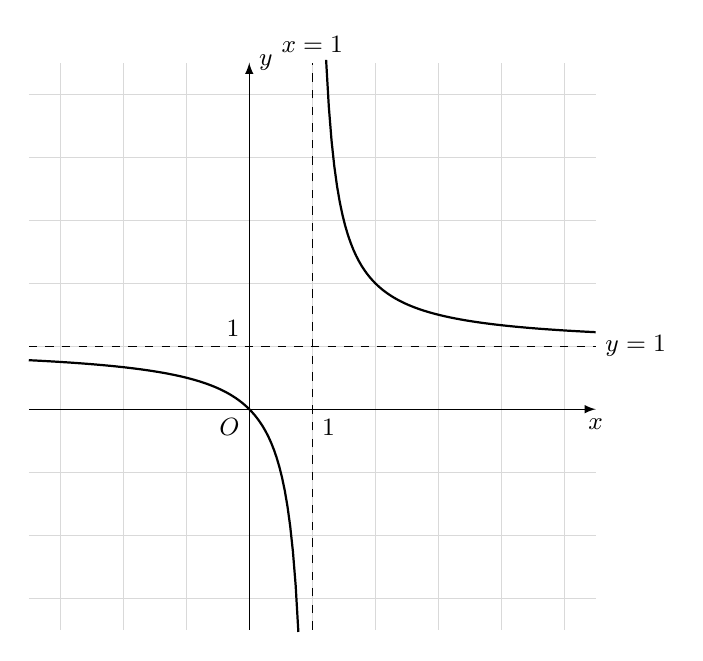
\begin{tikzpicture}[>=latex, scale=0.8]
    % 1. Vẽ lưới
    \draw[color=gray!30, thin, step=1] (-3.5,-3.5) grid (5.5,5.5);
    
    % 2. Vẽ hệ trục tọa độ
    \draw[->] (-3.5,0) -- (5.5,0) node[below] {\small $x$};
    \draw[->] (0,-3.5) -- (0,5.5) node[right] {\small $y$};
    \node[below left] at (0,0) {\small $O$};
    
    % 4. Vẽ đồ thị hàm số y = x/(x-1)
    \draw[thick, samples=100, domain=-3.5:0.78] 
        plot (\x, {\x/(\x - 1)});
    \draw[thick, samples=100, domain=1.22:5.5] 
        plot (\x, {\x/(\x - 1)});
    
    % 5. Đường tiệm cận
    \draw[dashed] (1,-3.5) -- (1,5.5) node[above] {\small $x=1$};
    \draw[dashed] (-3.5,1) -- (5.5,1) node[right] {\small $y=1$};
    \node[below right] at ( 1,0) {\small $1$};
    \node [ above left] at (0,1) {\small $1$};
\end{tikzpicture}
\end{center}

}{
    \begin{tasks}(4)
        \task \( y = \dfrac{x}{x+1} \)
        \task \( y = -\dfrac{x}{x-1} \)
        \task \( y = -\dfrac{x}{x+1} \)
        \task \( y = \dfrac{x}{x-1} \)
    \end{tasks}
}

% --- CÂU 10 ---
\questionLinesManual{5}{3}{Đường cong ở hình dưới đây là đồ thị của hàm số

\begin{center}
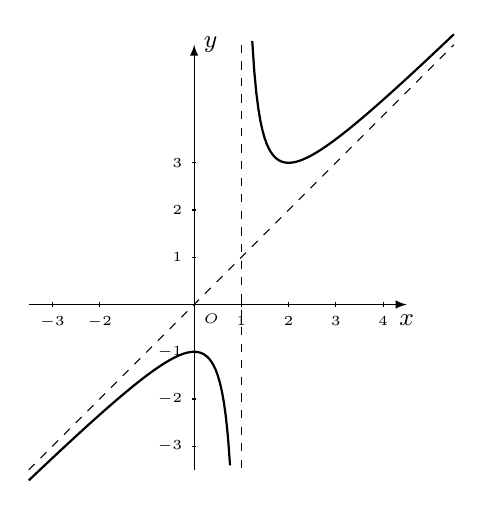
\begin{tikzpicture}[>=latex, scale=0.6]
    \draw[->] (-3.5,0) -- (4.5,0) node[below] {\small $x$};
    \draw[->] (0,-3.5) -- (0,5.5) node[right] {\small $y$};
    \node[below right] at (0,0) {\tiny $O$};
    
    % 3. Đánh dấu các mốc
    \foreach \x in {-3,-2,1,2,3,4} {
        \draw (\x,0.05) -- (\x,-0.05) node[below] {\tiny $\x$};
    }
    \foreach \val in {-3,-2,-1,1,2,3} {
        \draw (0.05,\val) -- (-0.05,\val) node[left] {\tiny $\val$};
    }
    
    % 4. Vẽ đồ thị hàm số y = (x^2 - x + 1)/(x - 1)
    \draw[thick, samples=100, domain=-3.5:0.76] 
        plot (\x, {(\x*\x - \x + 1)/(\x - 1)});
    \draw[thick, samples=100, domain=1.23:5.5] 
        plot (\x, {(\x*\x - \x + 1)/(\x - 1)});
    
    % 5. Đường tiệm cận
    \draw[dashed] (1,5.5) -- (1,-3.5) ;
    \draw[dashed] (-3.5,-3.5) -- (5.5,5.5) ;
\end{tikzpicture}
\end{center}

}{
    \begin{tasks}(4)
        \task \( y = \dfrac{x^2 - 4x + 5}{x - 2} \)
        \task \( y = \dfrac{x^2 - 4x - 1}{x + 1} \)
        \task \( y = \dfrac{x^2 - x + 1}{x - 1} \)
        \task \( y = \dfrac{x^2 + x - 1}{x - 1} \)
    \end{tasks}
}

\questionLinesManual{5}{4}{Đường cong trong hình vẽ là đồ thị của hàm số nào dưới đây?

\begin{center}
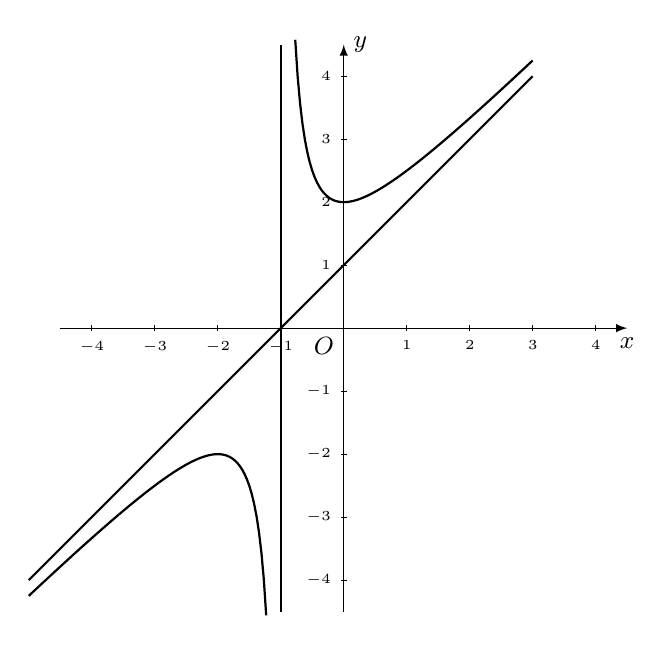
\begin{tikzpicture}[>=latex, scale=0.8]
    % 1. Hệ trục tọa độ
    \draw[->] (-4.5,0) -- (4.5,0) node[below] {\small $x$};
    \draw[->] (0,-4.5) -- (0,4.5) node[right] {\small $y$};
    \node[below left] at (0,0) {\small $O$};
    
    % 2. Đánh dấu các mốc
    \foreach \x in {-4,-3,-2,-1,1,2,3,4} {
        \draw (\x,0.05) -- (\x,-0.05) node[below] {\tiny $\x$};
    }
    \foreach \val in {-4,-3,-2,-1,1,2,3,4} {
        \draw (0.05,\val) -- (-0.05,\val) node[left] {\tiny $\val$};
    }
    
    % 3. Vẽ đồ thị hàm số y = (x^2 + 2x + 2)/(x + 1)
    \draw[thick, samples=100, domain=-5:-1.23] 
        plot (\x, {(\x*\x + 2*\x + 2)/(\x + 1)});
    \draw[thick, samples=100, domain=-0.77:3] 
        plot (\x, {(\x*\x + 2*\x + 2)/(\x + 1)});
    \draw[thick, samples=100, domain=-5:3] 
        plot (\x, {\x+1});
    
    % 4. Đường tiệm cận
    \draw[thick] (-1,-4.5) -- (-1,4.5);
\end{tikzpicture}
\end{center}

}{
    \begin{tasks}(4)
        \task \( y = \dfrac{x^2 + 2x + 2}{x + 1} \)
        \task \( y = \dfrac{x^2 - 2x - 3}{x - 2} \)
        \task \( y = \dfrac{x^2 + 3x}{x - 2} \)
        \task \( y = \dfrac{x^2 - 2x}{x + 1} \)
    \end{tasks}
}

\newpage
\drawdashlines{25}

\questionLinesManual{12}{5}{Cho hàm số \( y = \dfrac{ax + b}{cx + d} \) có đồ thị như trong hình bên dưới. Biết rằng \( a \) là số thực dương, hỏi trong các số \( b, c, d \) có tất cả bao nhiêu số dương?

\begin{center}
\begin{tikzpicture}[>=latex, scale=0.8]
    % Vẽ hệ trục
    \draw[->] (-5.5,0) -- (3.5,0) node[below] {$x$};
    \draw[->] (0,-2.5) -- (0,6.5) node[right] {$y$};
    \node[below left] at (0,0) {$O$};
    % Vẽ đồ thị hàm số
    \draw[thick, samples=100, domain=-5.5:-1.7] 
        plot (\x, {(2*\x - 1)/(\x + 1)});
    \draw[thick, samples=100, domain=-0.35:3.5] 
        plot (\x, {(2*\x - 1)/(\x + 1)});
    
    % Đường tiệm cận
    \draw[dashed] (-1,-2.5) -- (-1,6.5);
    \draw[dashed] (-5.5,2) -- (3.5,2);
\end{tikzpicture}
\end{center}

}{
    \begin{tasks}(4)
        \task $1$
        \task $2$
        \task $0$
        \task $3$
    \end{tasks}
}

\questionLinesManual{12}{6}{Cho hàm số \( y = \dfrac{ax + b}{cx + d} \) có đồ thị như sau.

\begin{center}
\begin{tikzpicture}[>=latex, scale=0.8]
    % Vẽ hệ trục
    \draw[->] (-3.5,0) -- (5.5,0) node[below] {$x$};
    \draw[->] (0,-3.5) -- (0,5.5) node[right] {$y$};
    \node[below right] at (0,0) {$O$};
   
    % Vẽ đồ thị hàm số
    \draw[thick, samples=100, domain=-3.5:0.55] 
        plot (\x, {(\x + 1)/(\x -1)});
    \draw[thick, samples=100, domain=1.45:5.5] 
        plot (\x, {(\x + 1)/(\x - 1)});
    
    % Đường tiệm cận
    \draw[dashed] (1,-3.5) -- (1,5.5) ;
    \draw[dashed] (-3.5,1) -- (5.5,1);
\end{tikzpicture}
\end{center}

Mệnh đề nào sau đây đúng?}{
    \begin{tasks}(4)
        \task \( ac > 0; \, bd > 0 \)
        \task \( ab < 0; \, cd < 0 \)
        \task \( bc > 0; \, ad < 0 \)
        \task \( ad > 0; \, bd < 0 \)
    \end{tasks}
}



\questionLinesManual{12}{7}{Cho hàm số \( y = \dfrac{ax + b}{cx + d} \) có đồ thị như hình vẽ bên. Khẳng định nào sau đây là khẳng định đúng?

\begin{center}
\begin{tikzpicture}[>=latex, scale=0.5]
    % Vẽ hệ trục
    \draw[->] (-7.5,0) -- (4.5,0) node[below] {$x$};
    \draw[->] (0,-4.5) -- (0,6.5) node[right] {$y$};
    \node[below left] at (0,0) {$O$};
    
    % Vẽ đồ thị hàm số
    \draw[thick, samples=100, domain=-7.5:-2.55] 
        plot (\x, {(\x - 1)/(\x + 2)});
    \draw[thick, samples=100, domain=-1.45:4.5] 
        plot (\x, {(\x - 1)/(\x + 2)});
    
    % Đường tiệm cận
    \draw[dashed] (-2,-4.5) -- (-2,6.5);
    \draw[dashed] (-7.5,1) -- (4.5,1);
\end{tikzpicture}
\end{center}

}{
    \begin{tasks}(4)
        \task 
        \(\begin{cases} 
        ad < 0 \\ 
        bc > 0 
        \end{cases}\)
        \task 
        \(\begin{cases} 
        ad < 0 \\ 
        bc < 0 
        \end{cases}\)
        \task 
        \(\begin{cases} 
        ad > 0 \\ 
        bc < 0 
        \end{cases}\)
        \task 
        \(\begin{cases} 
        ad > 0 \\ 
        bc > 0 
        \end{cases}\)
    \end{tasks}
}

\questionLinesManual{15}{8}{Cho hàm số \( y = \dfrac{x^2 + bx + c}{mx + n} \) (\( m \neq 0 \))  có đồ thị là đường cong bên dưới

\begin{center}
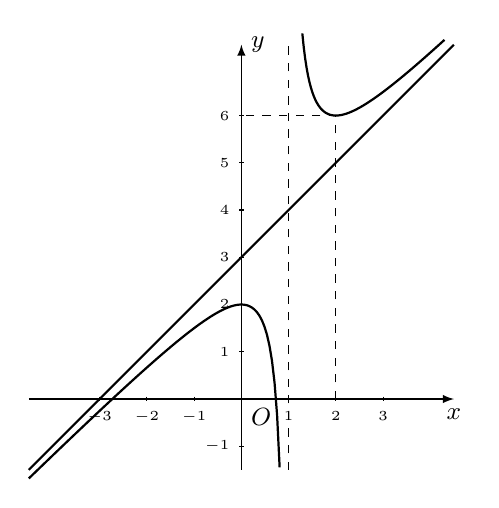
\begin{tikzpicture}[>=latex, scale=0.6]
    % 1. Hệ trục tọa độ
    \draw[->] (-4.5,0) -- (4.5,0) node[below] {\small $x$};
    \draw[->] (0,-1.5) -- (0,7.5) node[right] {\small $y$};
    \node[below right] at (0,0) {\small $O$};
    
    % 2. Đánh dấu các mốc
    \foreach \x in {-3,-2,-1,1,2,3} {
        \draw (\x,0.05) -- (\x,-0.05) node[below] {\tiny $\x$};
    }
    \foreach \val in {-1,1,2,3,4,5,6} {
        \draw (0.05,\val) -- (-0.05,\val) node[left] {\tiny $\val$};
    }
    
    % 3. Vẽ đồ thị hàm số y = (x^2 + x - 1)/(x - 1)
    \draw[thick, samples=100, domain=-4.5:0.81] 
        plot (\x, {(\x*\x - \x + 1)/(\x - 1)+3});
    \draw[thick, samples=100, domain=1.29:4.3] 
        plot (\x, {(\x*\x - \x +1)/(\x - 1)+3});
    \draw[thick, samples=100, domain=-4.5:4.5] 
        plot (\x, {(\x+3});
    % 4. Đường tiệm cận
    \draw[dashed] (1,-1.5) -- (1,7.5) ;
    \draw[dashed] (2,0) -- (2,6) -- (0,6);
\end{tikzpicture}
\end{center}

Trong các số \( b, c, m, n \) có tất cả bao nhiêu số dương?}{
    \begin{tasks}(4)
        \task $1$
        \task $2$
        \task $3$
        \task $4$
    \end{tasks}
}

\questionLinesManual{12}{9}{Cho hàm số \( y = \dfrac{ax^2 + bx + c}{x + d} \) (\( a \neq 0 \))  có đồ thị như hình vẽ sau:

\begin{center}
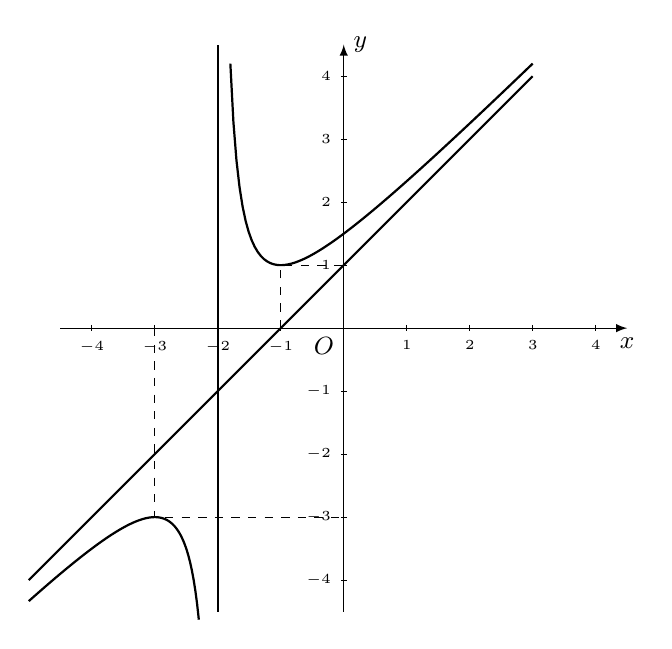
\begin{tikzpicture}[>=latex, scale=0.8]
    % 1. Hệ trục tọa độ
    \draw[->] (-4.5,0) -- (4.5,0) node[below] {\small $x$};
    \draw[->] (0,-4.5) -- (0,4.5) node[right] {\small $y$};
    \node[below left] at (0,0) {\small $O$};
    
    % 2. Đánh dấu các mốc
    \foreach \x in {-4,-3,-2,-1,1,2,3,4} {
        \draw (\x,0.05) -- (\x,-0.05) node[below] {\tiny $\x$};
    }
    \foreach \val in {-4,-3,-2,-1,1,2,3,4} {
        \draw (0.05,\val) -- (-0.05,\val) node[left] {\tiny $\val$};
    }
    
    % 3. Vẽ đồ thị hàm số y = (x^2 + 2x + 2)/(x + 1)
    \draw[thick, samples=100, domain=-5:-2.3] 
        plot (\x, {(\x*\x + 3*\x + 3)/(\x + 2)});
    \draw[thick, samples=100, domain=-1.8:3] 
        plot (\x, {(\x*\x + 3*\x + 3)/(\x + 2)});
    \draw[thick, samples=100, domain=-5:3] 
        plot (\x, {\x+1});
    
    % 4. Đường tiệm cận
    \draw[thick] (-2,-4.5) -- (-2,4.5);
    \draw [dashed] (-1,0) -- (-1,1) --(0,1);
    \draw[dashed] (-3,0) -- (-3,-3) --( 0,-3);
\end{tikzpicture}
\end{center}

Trong các số \( a, b, c, d \) có tất cả bao nhiêu số dương?}{
    \begin{tasks}(4)
        \task $1$
        \task $2$
        \task $3$
        \task $4$
    \end{tasks}
}

\questionLinesManual{12}{10}{Cho hàm số \( y = ax + b - \dfrac{r}{x} \) (\(ab  \neq 0\)) và có đồ thị là \( (C) \) có dạng như hình vẽ sau.

\begin{center}
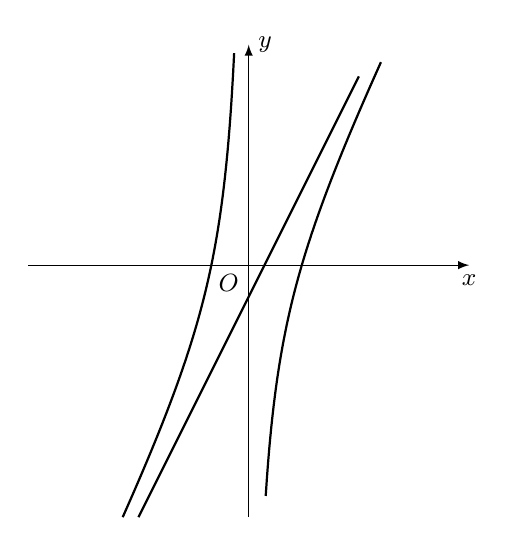
\begin{tikzpicture}[>=latex, scale=0.8]
    % 1. Hệ trục tọa độ
    \draw[->] (-3.5,0) -- (3.5,0) node[below] {\small $x$};
    \draw[->] (0,-4) -- (0,3.5) node[right] {\small $y$};
    \node[below left] at (0,0) {\small $O$};
   
    % 3. Vẽ đồ thị hàm số y = x + 1 - 2/x
    \draw[thick, samples=100, domain=-2:-0.23] 
        plot (\x, {2*\x  - 1/\x-0.5});
    \draw[thick, samples=100, domain=0.27:2.1] 
        plot (\x, {2*\x - 1/\x-0.5});
         \draw[thick, samples=100, domain=-1.75:1.75] 
        plot (\x, {2*\x-0.5 });
\end{tikzpicture}
\end{center}

Các hệ số \( a, b, r \) phải thỏa mãn điều kiện nào dưới đây.}{
    \begin{tasks}(4)
        \task 
        \(\begin{cases} 
        a > 0 \\ 
        b < 0 \\ 
        r > 0 
        \end{cases}\)
        \task 
        \(\begin{cases} 
        a > 0 \\ 
        b > 0 \\ 
        r < 0 
        \end{cases}\)
        \task 
        \(\begin{cases} 
        a < 0 \\ 
        b > 0 \\ 
        r > 0 
        \end{cases}\)
        \task 
        \(\begin{cases} 
        a > 0 \\ 
        b < 0 \\ 
        r < 0 
        \end{cases}\)
    \end{tasks}
}

\questionLinesManual{12}{11}{Cho hàm số \( y = \dfrac{ax + b}{x + c} \) có đồ thị như hình sau đây

\begin{center}
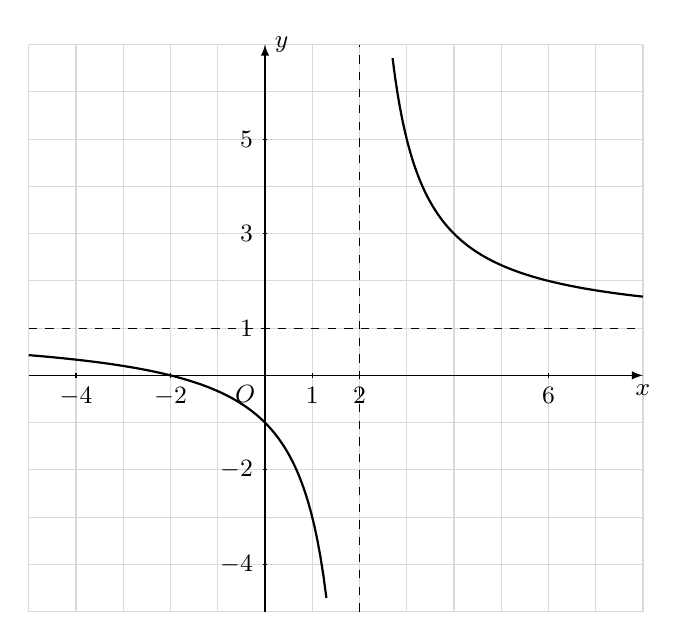
\begin{tikzpicture}[>=latex, scale=0.6]
    % 1. Vẽ lưới
    \draw[color=gray!30, thin, step=1] (-5,-5) grid (8,7);
    
    % 2. Vẽ hệ trục tọa độ
    \draw[->] (-5,0) -- (8,0) node[below] {\small $x$};
    \draw[->] (0,-5) -- (0,7) node[right] {\small $y$};
    \node[below left] at (0,0) {\small $O$};
    
    % 3. Đánh dấu các mốc
    \foreach \x in {-4,-2,1,2,6} {
        \draw (\x,0.05) -- (\x,-0.05) node[below] {\small $\x$};
    }
    \foreach \val in {-4,-2,1,3,5} {
        \draw (0.05,\val) -- (-0.05,\val) node[left] {\small $\val$};
    }
    
    % 4. Vẽ đồ thị hàm số y = (2x+1)/(x+1)
    \draw[thick, samples=100, domain=-5:1.3] 
        plot (\x, {(\x + 2)/(\x -2)});
    \draw[thick, samples=100, domain=2.7:8] 
        plot (\x, {(\x + 2)/(\x - 2)});
    
    % 5. Đường tiệm cận
    \draw[dashed] (2,-5) -- (2,7);
    \draw[dashed] (-5,1) -- (8,1);
\end{tikzpicture}
\end{center}

Tính giá trị của biểu thức \( P = 2a - b + 3c \).}{
    \begin{tasks}(4)
        \task $6$
        \task $-6$
        \task $10$
        \task $-2$
    \end{tasks}
}

\questionLinesManual{12}{12}{Cho hàm số \( y = \dfrac{ax^2 + bx + 1}{cx + 2} \) (với \( a, b, c \in \mathbb{R}, a \neq 0 \)) có đồ thị là đường cong trong hình vẽ bên. Giá trị biểu thức \( T = 2a + 3b - c \) là

\begin{center}
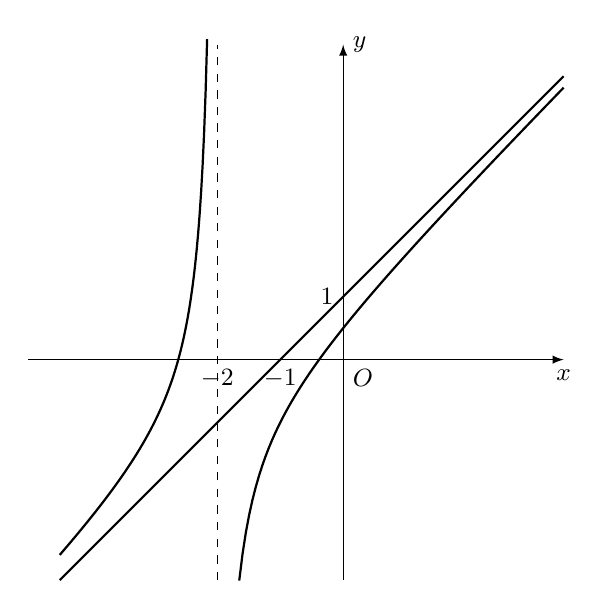
\begin{tikzpicture}[>=latex, scale=0.8]
    % 1. Hệ trục tọa độ
    \draw[->] (-5,0) -- (3.5,0) node[below] {\small $x$};
    \draw[->] (0,-3.5) -- (0,5) node[right] {\small $y$};
    \node[below right] at (0,0) {\small $O$};
    
    
    % 3. Vẽ đồ thị hàm số
    \draw[thick, samples=100, domain=-4.5:-2.16] 
        plot (\x, {\x+1 - 1/(\x + 2)});
    \draw[thick, samples=100, domain=-1.65:3.5] 
        plot (\x, {\x+1 - 1/(\x + 2)});
    \draw[thick, samples=100, domain=-4.5:3.5] 
        plot (\x, {\x+1 });
    % 4. Đường tiệm cận
    \draw[dashed] (-2,-3.5) -- (-2,5);
    \node [below] at (-2,0) {\small $-2$};
    \node [below] at (-1,0) {\small $-1$};
    \node [left] at (0,1) {\small $1$};
\end{tikzpicture}
\end{center}

}{
    \begin{tasks}(4)
        \task \( T = 11 \)
        \task \( T = 8 \)
        \task \( T = 9 \)
        \task \( T = 10 \)
    \end{tasks}
}

\questionLinesManual{3}{13}{Cho hàm số \( y = \dfrac{ax + b}{cx + d} \) (\(a, b, c \in \mathbb{R}\)) có đồ thị là đường cong như hình vẽ bên. Toạ độ tâm đối xứng của đồ thị hàm số đã cho là:

\begin{center}
\begin{tikzpicture}[>=latex, scale=0.8]
                % 1. Hệ trục tọa độ
                \draw[->] (-4.5,0) -- (3.5,0) node[below] {\small $x$};
                \draw[->] (0,-3.5) -- (0,4.5) node[right] {\small $y$};
                \node[below left] at (0,0) {\small $O$};
                
                % 2. Đánh dấu các mốc
                \foreach \x in {-1,1} {
                    \draw (\x,0.05) -- (\x,-0.05) node[below] {\small $\x$};
                }
                \foreach \val in {1} {
                    \draw (0.05,\val) -- (-0.05,\val) node[left] {\small $\val$};
                }
                
                % 3. Vẽ đồ thị hàm số y = (x+1)/(-x+1) = -(x+1)/(x-1)
                \draw[thick, samples=100, domain=-4.5:-1.57] 
                    plot (\x, {(\x - 1)/(\x + 1)});
                \draw[thick, samples=100, domain=-0.57:3.5] 
                    plot (\x, {(\x - 1)/(\x + 1)});
                
                % 4. Đường tiệm cận
                \draw[dashed] (-1,-3.5) -- (-1,4.5) ;
                \draw[dashed] (-4.5,1) -- (3.5,1) ;
            \end{tikzpicture}
\end{center}

}{
    \begin{tasks}(4)
        \task \((-1; 1)\)
        \task \((1; 1)\)
        \task \((1; -1)\)
        \task \((0; 1)\)
    \end{tasks}
}

\questionLinesManual{3}{14}{Cho hàm số \( y = \dfrac{ax^2 + bx + c}{mx + n} \) có đồ thị hàm số như hình vẽ:

\begin{center}
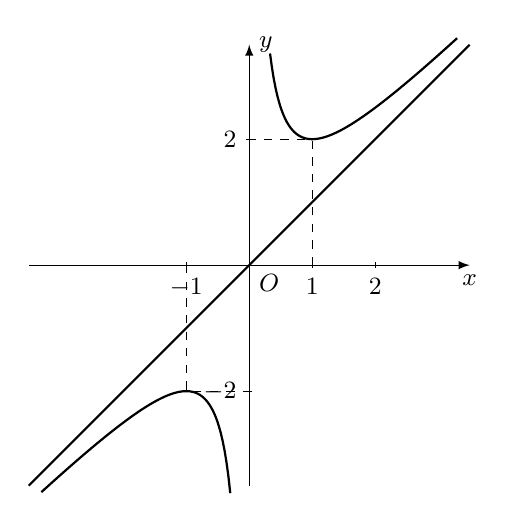
\begin{tikzpicture}[>=latex, scale=0.8]
    % 1. Hệ trục tọa độ
    \draw[->] (-3.5,0) -- (3.5,0) node[below] {\small $x$};
    \draw[->] (0,-3.5) -- (0,3.5) node[right] {\small $y$};
    \node[below right] at (0,0) {\small $O$};
    
    % 2. Đánh dấu các mốc
    \foreach \x in {-1,1,2} {
        \draw (\x,0.05) -- (\x,-0.05) node[below] {\small $\x$};
    }
    \foreach \val in {-2,2} {
        \draw (0.05,\val) -- (-0.05,\val) node[left] {\small $\val$};
    }
    
    % 3. Vẽ đồ thị hàm số
    \draw[thick, samples=100, domain=-3.3:-0.3] 
        plot (\x, {\x + 1/\x});
    \draw[thick, samples=100, domain=0.33:3.3] 
        plot (\x, {\x + 1/\x});
    \draw[thick, samples=100, domain=-3.5:3.5] 
        plot (\x, {\x });
        \draw[dashed] (1,0) -- (1,2)-- (0,2);
        \draw[dashed] (-1,0) -- (-1,-2) -- (0,-2);
\end{tikzpicture}
\end{center}

Tâm đối xứng của đồ thị hàm số đã cho là}{
    \begin{tasks}(4)
        \task \( I(1; 2) \)
        \task \( J(-1; -2) \)
        \task \( K(1; 1) \)
        \task \( O(0; 0) \)
    \end{tasks}
}

\questionLinesManual{5}{15}{Cho hàm số \( y = -2x^3 + 6x^2 - 4x + 1 \). Tâm đối xứng của đồ thị hàm số có tạo độ bằng:}

\questionLinesManual{5}{16}{Cho hàm số \( y = \dfrac{2x + 1}{x - 1} \). Tâm đối xứng của đồ thị hàm số là:}

\questionLinesManual{5}{17}{Cho hàm số \( y = \dfrac{x^2 + 2x + 2}{x + 1} \). Tâm đối xứng của đồ thị hàm số là:}

\questionLinesManual{8}{18}{Phương trình tiếp tuyến của đồ thị hàm số \( y = \dfrac{x - 2}{x + 1} \) tại điểm có hoành độ \(x_0 = -2\) là}

\questionLinesManual{8}{19}{Cho hàm số \( y = \dfrac{x^2 + 3x + 3}{x + 1} \) có đồ thị \((C)\). Tiếp tuyến của đồ thị \((C)\) tại \(x_0 = 0\)}

\questionLinesManual{8}{20}{Đường thẳng qua 2 điểm cực trị của đồ thị hàm số \( y = \dfrac{x^2 - x + 2}{x + 2} \) có phương trình là}

\newpage
\drawdashlines{25}


\end{document}